\documentclass{article}
\usepackage[utf8]{inputenc}
\usepackage[dutch]{babel}
\usepackage[square,sort,comma,numbers]{natbib}
\usepackage[hyphens]{url}
\usepackage{tikz}
\usetikzlibrary{trees}
\usepackage{float}
\usepackage{hyperref}
\setlength
{\parindent}
{0pt}
\setlength
{\parskip}
{1.5ex plus 0.5ex minus 0.2ex}
\usepackage[margin=3.5cm]{geometry}


\title{Artificiële Intelligentie: Opdracht 2 (Constraint Processing)}
\author{Mathias Van Herreweghe - r0456156}
\date{3 december 2014}

\usepackage{natbib}
\usepackage{graphicx}

\begin{document}

\maketitle
\newpage

\section{Opgave}
Het nieuwe academiejaar begint en je bent op zoek naar een nieuwe verblijfplaats. Een vriend vertelt je dat er een huis met vijf kamers te huur staat in Heverlee. Alle kamers bevinden zich op de gelijkvloers en liggen op één rij naast elkaar, kamer 1 ligt helemaal links in het gebouw, kamer 5 helemaal rechts. De vriend vindt na even zoeken nog drie andere personen om een kamer te huren. De ingang van het huis is aan kamer 1. In totaal zijn er dus vijf personen in het huis. Natuurlijk is het een gekibbel en gedoe om de kamers te kiezen tussen de vijf personen. Men wilt namelijk dat onder andere de volgende eigenschappen voldaan zijn:


\begin{itemize}
\item persoon 1 gaat vaak in en uit zijn kamer en wilt dus niet meer dan 3 kamers verwijderd zijn van de ingang aan kamer 1, ook wilt persoon 1 een kamer naast persoon 2,
\item persoon 2 wil niet in kamer 5 omdat deze te dicht bij de spoorweg ligt 10 meter verder, ook wilt persoon 2 een kamer die minstens 2 kamernummers groter is dan die van persoon 5,
\item persoon 3 kan niet tegen de tocht van de ingang en wil dus meer dan 2 kamers verwijderd zijn van de ingang aan kamer 1, ook wilt persoon 3 een kamer naast de kamer van persoon 4,
\item persoon 4 denkt dat er veel last hebt van lawaai als je in de middelste kamer ligt en wil dus niet in kamer 3, ook wilt persoon 4 exact twee kamernummers verschil tussen diens kamernummer en die van persoon 2,
\item persoon 5 wilt een kamernummer kleiner dan die van persoon 1,
\item ten slotte spreekt het voor zich dat er geen kamers gedeeld worden tussen personen.
\end{itemize}

Nu is het een jou, de wetenschapper, om hier een oplossing voor te vinden.

\newpage
\section{Model oplossing}

De waarde van elke kamer is de kamernummer zelf. De kamer-nummering begint bij 1, zijnde de meest linkse kamer en stopt bij kamernummer 5 (de meest rechtse kamer). We nemen $z_{p1}$, $z_{p2}$, $z_{p3}$, $z_{p4}$ en $z_{p5}$ voor de kamernummer van respectievelijk persoon 1 tot en met persoon 5.

\subsection{Unaire constraints}
We halen eerst de unaire constraints uit de eisen van de verschillende personen.

Ten eerste wilt persoon 1 een kamer dat niet meer dan 3 kamernummers verschilt van de ingang (kamernummer 1).
\[
z_{p1} < 4
\]

Vervolgens wilt Persoon 2 niet in kamer 5.
\[
z_{p2} \neq 5
\]

Daarnaast wilt persoon 3 een kamer dat minstens 2 kamernummers verschilt van de ingang (kamernummer 1).
\[
z_{p3} > 2
\]

Ten slotte wilt persoon 4 niet in kamer 3.
\[
z_{p4} \neq 3
\]

We bekomen de volgende unaire constraints.
\[
\left\lbrace
\begin{array}{c c c}
c(z_{p1}) & \leftrightarrow & z_{p1} < 4\\
c(z_{p2}) & \leftrightarrow & z_{p2} \neq 5\\
c(z_{p3}) & \leftrightarrow & z_{p3} > 2\\
c(z_{p4}) & \leftrightarrow & z_{p4} \neq 3\\
c(z_{p5}) & \leftrightarrow & \textbf{true}\\
\end{array}
\right.
\]

\newpage
\subsection{Binaire constraints}
Verder zijn er nog binaire constraints gegeven, deze drukken we formeel uit zoals volgt.

Persoon 1 wilt een kamer naast die van persoon 2.
\[
|z_{p1} - z_{p2}| = 1
\]

Persoon 2 wilt een kamer met minstens 2 kamernummers groter dan die van persoon 5.
\[
z_{p2} - z_{p5} > 1
\]

Persoon 3 wilt een kamer naast die van persoon 4.
\[
|z_{p3} - z_{p4}| = 1
\]

Persoon 3 wilt een kamer met minstens 2 kamernummers verschil met die van persoon 1.
\[
|z_{p3} - z_{p1}| > 1
\]

Persoon 4 wilt exact 2 kamernummers verschil tussen diens kamernummer en die van persoon 2.
\[
|z_{p4} - z_{p2}| = 2
\]

Persoon 5 wilt een kamernummer kleiner dan die van persoon 1.
\[
z_{p5} < z_{p1}
\]

We bekomen de volgende binaire constraints.
\[
\left\lbrace
\begin{array}{c c c c l}
c(z_{p1}, z_{p2}) & \leftrightarrow & z_{p1} \neq z_{p2} & \wedge & |z_{p1} - z_{p2}| = 1\\
c(z_{p1}, z_{p3}) & \leftrightarrow & z_{p1} \neq z_{p3}\\
c(z_{p1}, z_{p4}) & \leftrightarrow & z_{p1} \neq z_{p4}\\
c(z_{p1}, z_{p5}) & \leftrightarrow & z_{p1} \neq z_{p5} & \wedge & z_{p5} < z_{p1}\\
c(z_{p2}, z_{p3}) & \leftrightarrow & z_{p2} \neq z_{p3}\\
c(z_{p2}, z_{p4}) & \leftrightarrow & z_{p2} \neq z_{p4} & \wedge & |z_{2} - z_{p4}| = 2\\
c(z_{p2}, z_{p5}) & \leftrightarrow & z_{p2} \neq z_{p5} & \wedge & z_{p2} - z_{p5} > 1\\
c(z_{p3}, z_{p4}) & \leftrightarrow & z_{p3} \neq z_{p4} & \wedge & |z_{p3} - z_{p4}| = 1\\
c(z_{p3}, z_{p5}) & \leftrightarrow & z_{p3} \neq z_{p5}\\
c(z_{p4}, z_{p5}) & \leftrightarrow & z_{p4} \neq z_{p5}\\


\end{array}
\right.
\]

\newpage
\subsection{Domein}
Aanvankelijk heeft elke variabele het domein $d_i = {1,2,3,4,5}$. Door de unaire constraints toe te passen kunnen we de domeinen beperken. Het toepassen van de unaire constraints doen we volgens  $d'_i = \{a|a \in d_i \wedge c(z_i = a)\}$.

\[
\left\lbrace
\begin{array}{c l}
d_{z_{p1}}' &= \{1,2,3\}\\
d_{z_{p2}}' &= \{1,2,3,4\}\\
d_{z_{p3}}' &= \{3,4,5\}\\
d_{z_{p4}}' &= \{1,2,4,5\}\\
d_{z_{p5}}' &= \{1,2,3,4,5\}\\
\end{array}
\right.
\]

\subsection{Constraint network}

\begin{figure}[H]
\caption{Constraint Network}
\label{constraint_network}
\centering
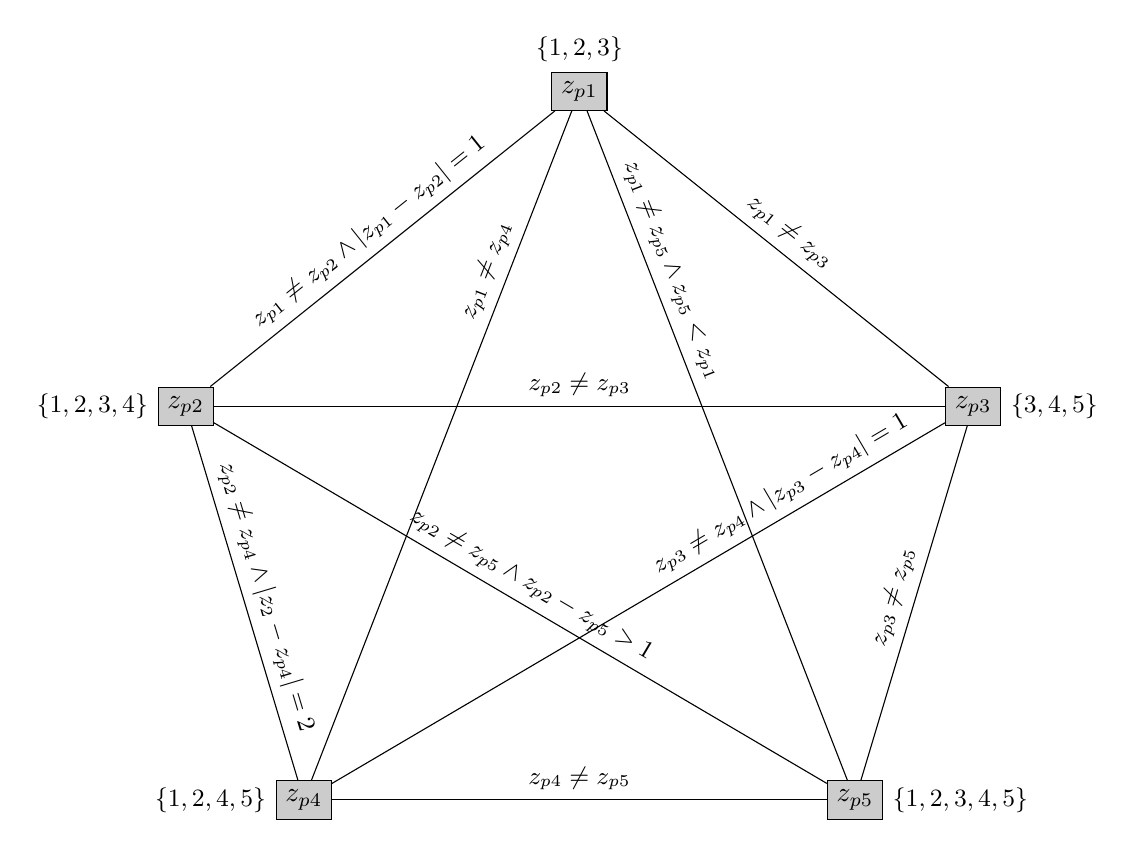
\begin{tikzpicture}[vari/.style={fill=black!20,rectangle,draw=black}]
\node[vari] (A) at (0,4) {$z_{p1}$};
\node[vari] (B) at (-5,0) {$z_{p2}$};
\node[vari] (C) at (5,0) {$z_{p3}$};
\node[vari] (D) at (-3.5,-5) {$z_{p4}$};
\node[vari] (E) at (3.5,-5) {$z_{p5}$};

\node[anchor=south] (dA) at (A.north) {\small{$\left\{1,2,3\right\}$}};
\node[anchor=east] (dB) at (B.west) {\small{$\left\{1,2,3,4\right\}$}};
\node[anchor=west] (dC) at (C.east) {\small{$\left\{3,4,5\right\}$}};
\node[anchor=east] (dD) at (D.west) {\small{$\left\{1,2,4,5\right\}$}};
\node[anchor=west] (dE) at (E.east) {\small{$\left\{1,2,3,4,5\right\}$}};

\draw (A) to node[midway,sloped,above]{\small{$z_{p1} \neq z_{p2} \wedge |z_{p1} - z_{p2}| = 1$}} (B); %12
\draw (A) to node[midway,sloped,above]{\small{$z_{p1} \neq z_{p3}$}} (C); %13
\draw (A) to node[near start,sloped,above]{\small{$z_{p1} \neq z_{p4}$}} (D); %14
\draw (A) to node[near start,sloped,above]{\small{$z_{p1} \neq z_{p5} \wedge z_{p5} < z_{p1}$}} (E); %15
\draw (B) to node[midway,sloped,above]{\small{$z_{p2} \neq z_{p3}$}} (C); %23
\draw (B) to node[midway,sloped,above]{\small{$z_{p2} \neq z_{p4} \wedge |z_{2} - z_{p4}| = 2$}} (D); %24
\draw (B) to node[midway,sloped,above]{\small{$z_{p2} \neq z_{p5} \wedge z_{p2} - z_{p5} > 1$}} (E); %25
\draw (C) to node[near start,sloped,above]{\small{$z_{p3} \neq z_{p4} \wedge |z_{p3} - z_{p4}| = 1$}} (D); %34
\draw (C) to node[midway,sloped,above]{\small{$z_{p3} \neq z_{p5}$}} (E); %35
\draw (D) to node[midway,sloped,above]{\small{$z_{p4} \neq z_{p5}$}} (E); %45

\end{tikzpicture}
\end{figure}
Het probleem kan men voorstellen door een constraint network, dit zie je op figuur \ref{constraint_network}.

\newpage
\subsection{Uitwerking van het probleem}
We maken gebruik van Dynamic Search Rearrangement met het First-Fail principle, we kiezen steeds de variabele met het kleinste domein. Indien het domein even groot is kiezen we tussen deze variabelen, de variabele met de meeste non-trivial constraints. Je vindt de uitwerking op Figuur \ref{uitwerking}.

\newpage
\begin{figure}[H]
\caption{Uitwerking}
\label{uitwerking}
\centering
\includegraphics[scale=0.135, angle=90]{uitwerking.jpg}
\end{figure}

\end{document}
